\chapter{Introduction}\label{chap:introduction}
Unmanned Aerial Vehicles (UAVs) are, nowadays, accessible to all kind of users and many applications have been trying to use these vehicles in more and more difficult settings. For many of these scenarios it is necessary an autonomous landing of the UAV on a platform using only onboard sensors. As a matter of fact one of the major drawback of current civil Micro Air Vehicles (MAVs) is the limited flight time: automated landing systems (along with suitable recharging platforms) enable longer UAV missions with greater autonomy.\\
Furthermore, it is highly possible, that a these applications require the landing target to be moving, for example it can be a car during a reconnaissance, so the MAV must be able to perform a precise landing maneuver over a specific moving platform.\\

Highly accurate localization is required in order to allow the MAV to land precisely over the platform. Most of UAVs are equipped with a GPS, but this sensor can have errors up to 5 meters radius, and landing with such low-quality state estimation will have an almost certain probability of failure. Fortunately, many applications require the usage of other sensors, such as onboard cameras: vision based approaches, to estimate the state both of the UAV and of the moving base, are promising in this respect.\\

In this work we present a complete framework to perform an entire landing task. The main parts of the framework are:
\begin{itemize}
\item self localization and state estimation of the UAV.
\item detection, tracking and state estimation of the landing target.
\item dynamic trajectory planning to perform a precise and smooth land over the target.
\end{itemize}

\section{Related Work}\label{sec:related_work}

During the last 15 years several methods where developed in order to achieve automatic landing for UAVs.
Usually, in these projects, calculations are done by ground stations, which allows great processing power, but leads to restrictions in autonomy on the UAV. \\

At the beginning the research was focused on landing on a static platform. \\
Hardware and techniques used to achieve the successful completion of the task were various.

Some of them, like Saripalli in \cite{saripalli2002vision}, presents a vision-based autonomous landing algorithm using big vehicles that can carry industrial sensors and high performance processors. This work uses hardware very far from the one we want to use, but it one of the first approaches to find a solution of this problem.

Other works, like Sharp in \cite{sharp2001vision} and Lange in \cite{lange2008autonomous}, are using little UAVs with cameras, but they are estimating the pose of the quadrotor only w.r.t the landing base, that consists on a single tag, so these frameworks are not robust to the loss of the tag and to the noise introduced using just a single reference for the state estimation.\\ 
Another similar work is done by Herisse in \cite{herisse2008hovering}, where only optical flow information is used for hovering flight and vertical landing control.\\
All these framework works correctly but the main difference with our approach is that their frameworks consist just in the landing maneuver and so the final target is always in the f.o.v. of the camera, an assumption that for as is not possible to do.

Other papers present promising theoretical algorithm to perform a smooth and precise landing, but only tested in simulation, like Tang in \cite{tang2011uav} where it develop a landing framework based on N-points algorithm and orthogonalization to estimate the state of the aircraft, or like Jiang in \cite{jian2012automatic} where he developed a theoretical optical guided landing control system and its corresponding guidance control law.\\



More interesting for the purpose of this thesis, are researches about landing on a moving platform.

Wenzel in \cite{wenzel2011automatic} is performing tracking and landing on a moving base with a small quadrotor. All the experiments are in inside environment, because he is using IR camera, sensors not robust to outside conditions, which allows robust tracking of a pattern of IR lights without direct sunlight. It achieve precise and consistent results with a platform moving both in a circular path or emulating a ship turning on water, but the movement is not fast, $0.4m/s$.

Lee in \cite{lee2012autonomous} is using visual servoing to perform the landing maneuver: they develop a feedback control based on the position of the target in the camera image, this idea is interesting because we can always assume that the landing platform has some distinctive features to use to identify the final position where the UAV should go in order to properly land.\\
Also in this case the landing base is moving slow $0.07m/s$ and is moving always in a straight line. To control the quadrotor to the landing site they are using a Sliding Mode Control, this method can deal with non linearity of the dynamics and external modeled noise (like the model of the ground effect force). 

Kim in \cite{Kim2016} uses color filter to find the landing target, the platform has a color unique in the environment and this feature can be spoil to find it easily, furthermore he uses an omnidirectional camera to have always the target in the field of view. Given the measurement of the position of the camera he implements an Extended Kalman Filter to filter the noise and predict the future position of the target. When the state of the moving base it is estimate, the knowledge of the type of movement the platform is performing, can be crucial in order to filter noisy measures and predict where the target will be within $t$ seconds. Once the future position is calculate a trajectory, in position and velocity, is computed from the initial pose of the quadrotor to the final intersection point. A velocity-attitude control is implement to follow the trajectory, and the precomputed trajectory is followed until the end, without replanning.

Mellinger in \cite{mellinger2010control} is addressing another type of problem: landing on tilted surface in which the quadrotor must pearch. He uses  motion capture system in order to have both UAV and target state estimation. His algorithm consists 
in a precomputed trajectory followed by a position-altitude control based on the linearized system of the quadrotor.\\
An interesting part of this work is the subdivision of the task in smaller parts in which trajectories and control are different in order to increase the robustness of the whole maneuver.

Vlantis in \cite{vlantis2015quadrotor} studied the problem of landing a quadrotor on an inclined moving platform. The UAV carries a forward looking camera to detect and observe the landing platform. In order to complete the task he developed a discrete-time non-linear Model Predictive Controller \cite{camacho2013model}  that optimizes both the trajectories and the time horizon, while respecting input and state constraints (not collide with the platform).\\ 
The cost function of the MPC consists in different factors weighted with dynamic coefficients (function of the relative position between UAV and moving platform). There are classical therms related to the time, the state of the quadrotor (position, orientation, velocity, body-rates), the smoothness and aggressiveness of the control inputs, and other factors regarding the landing task, such as: the alignment between the states of UAV and moving platform (relative position, orientation, velocity) and the fact that the center of the platform should be kept within the camera's field of view during the approaching phase.\\
This method seems really effective, but the major drawback of this approach is that the MPC is computationally very expensive and it is not possible to run the algorithm on-board: it is necessary a ground station that carries the huge amount of calculation that MPC requires.\\

The main conclusions from the analysis of these related works is that to design a landing framework we need:
\begin{itemize}
\item a good estimation of the UAV's state and moving platform's state.
\item a "manager" that considering the state estimations define a current stage of the system, and assign a specific task for this phase.
\item a MPC-like algorithm that control the quadrotor to complete the task assigned, the algorithm should increase the robustness updating continuously the future actions that must be applied to the UAV.
\end{itemize}


Several papers have been written on MPC applied to control of the quadrotor.

In \cite{neunertfast} Neunert et.al. present a framework for real-time, unconstrained, nonlinear MPC. The algorithm combines trajectory optimization and tracking control in a unified approach. It solves the MPC problem using repeatedly a method colled Sqeuqntial Linear Quadratic (explained in \cite{sideris2005efficient}), generating feedforward and feedback controls actions. This method allows agile flight maneuvers with accurate tracking. All the calculations are made on an on-board i7 CPU achieving a rate slightly below $40Hz$. The major drawback for us is that we have also perform many other computations on the on-board computer, so it is not possible to reach this frequency in the controller.

In the paper \cite{bangura2014real} Bangura presents a solution to on-board trajectory tracking control of quadrotors. The
proposed approach combines a standard control paradigm for attitude and a high-level trajectory tracking with a MPC strategy. 
In order to reduce the complexity, the system is feedback linearized obtaining an equivalent linear model to which the MPC framework can be applied. Also in this case only the computation related to MPC are computed onboard.

Mueller in \cite{mueller2013model} and later in \cite{mueller2015computationally} presents a method for rapid generation and feasibility verification of trajectories for quadrotors. The motion primitives are defined by the quadrotor's initial state, at time $t_0$ (position, velocity, acceleration), the desired motion duration $T$, and any combination of components of the quadrotor's
position, velocity and acceleration at time $t_0+T$. The trajectory are the solution of the optimization problem which minimize a
cost function related to input aggressiveness, and checks if it is feasible both with respect to input and state constraints. Million motion primitives may be evaluated and compared per second, and so the best feasible one can be picked and followed.\\


This final paper is very promising for our purpose because our problem can be exactly be expressed as the one solved by the algorithm proposed, and also because it is computationally inexpensive and so it is possible to run the entire code directly onboard.\\ Furthermore it is possible to use this code in an MPC-style: we have a controller with rate $\frac{1}{dt}$, at initial time $t_0$ the entire trajectory (from $t_0$ to $t_0 + T$) is calculated but only the first desired state of the trajectory (related to time $t_0+dt$) is considered, then at the next control cycle we repeat the procedure calculating the trajectory from $t_0 + dt$ to $t_0 + T$, and so on.

The following table summarizes the work done in previous research on this topic.

{
\newcolumntype{P}[1]{>{\centering\arraybackslash}p{#1}}
\definecolor{my_red}{rgb}{0.6350, 0.0780 ,0.1840}
\definecolor{my_green}{rgb}{0,0.5, 0}
\newcommand{\cmark}{\color{my_green} \ding{51}}
\newcommand{\xmark}{\color{my_red} \ding{55}}


\begin{center}
    \begin{tabular}{|p{4.2cm}|P{1.4cm}|P{1.4cm}|P{1.4cm}|P{1.4cm}|}
    \hline
                                                      &\color{black}\textbf{Lee} 2012  &\color{black} \textbf{Wenzel} 2011  &\color{black} \textbf{Kim} 2016 & \color{black}\textbf{Vlantis} 2015\\ \hline
    \color{black}\textbf{velocity platform} [m/s] & \color{my_red}  \textbf{0.07} & \color{my_red} \textbf{0.4} & \color{my_red} \textbf{0.5} & \color{my_red} \textbf{0.5} \\ \hline
   \color{black}\textbf{outdoor testing}             & \xmark     & \xmark         & \cmark     & \cmark \\ \hline
   \color{black}\textbf{quad indip. state estim.}     & \xmark     & \xmark         & \cmark     & \cmark \\ \hline
   \color{black} \textbf{platform dynamics}    & \xmark    & \xmark         & \cmark     & \cmark \\ \hline
    \color{black}\textbf{replanning}                   & \xmark    & \xmark          & \xmark    & \cmark \\ \hline
   \color{black}\textbf{onboard computation}  & \xmark    & \cmark          & \xmark      &\xmark \\
    \hline
    \end{tabular}
\end{center}
}

%Nonlinear Tracking and landing controller for quadrotor aerial robots
%Attitude - velocity controllers
%Attitude controller: with the desired angles calculate ui* with linear eq and then nonlinear control ui from eq (8) 
%Velocity control: given desired velocity computes the desired angles and control u1 with nonlinear function (12-15)
%Model with also gyroscopic torques of the rotors then neglected
%Dynamic of the angles approximate with roll, pitch and yaw little??
%Feedback linearize 
%Landing with two different control-landing (height of base and its velocities considered as disturbances)
%z direction -> stabilize the uav at a setpoint (approach 5m, then 0m) PD controller linear
%x,y plane distance -> 0 knowing velocity x-y of the base, distance and angle between the two body frames calculate nonlinear %control  (24-25) that brings system to converge to the desired point, this control are velocity in x-y direction to give to velocity control\\

%Feedback Linearization vs. Adaptive Sliding Mode Control for a Quadrotor Helicopter 
%Need adaptive control to compensate ground effect (unknown perturbation)
%Feedback linearization
%Sliding model control to compensate the ground effect uncertantain

%Precise Quadrotor Autonomous Landing with SRUKF Vision Perception
%Not very interesting, only estimation part, controller is done with PID without any new stuffs near the ground they only estimate the velocity of the quadrotor and no the position, because the second one is difficult (easy to lose the tag)

%Coordinate landing of a quadrotor on a skid-steered ground vehicle in the presence of time delays
%Their model of the UAV dynamics are incomplete for the angular accelerations
%Control both UAV and vehicle on the ground
%Feedback linearize the system define as output x,y,x,psi
%Joint decentralized control -> exponential stabilization of the particular set of dynamics to drive relative position error to 0


\section{MBZIRC challenge}\label{chap:thechallenge}
The main reason for the development of this thesis is the participation in the Mohamed Bin Zayed International Robotics Challenge \cite{challenge_description}. MBZIRC is an international robotics competition, held every two years, that provides an ambitious and technologically demanding set of challenges, that aim to inspire the future of robotics.\\ 
In the description of the competition they motivate the challenge claiming that robotics have an increasing impact in a variety of new markets and on various human social aspects (for example disaster response, oil and gas, manufacturing, construction and household chores) and MBZIRC should lay the foundations of technologies for such applications include robots working more autonomously in dynamic, unstructured environments, while collaborating and interacting with other robots and humans. \\

The competition is composed of 3 challenges and in this thesis we develop a framework to complete challenge number 1 which consists in an UAV landing on a moving ground vehicle. 
The specifications of the challenge are:
\begin{itemize}
\item Duration: 20 minutes.
\item UAV initial condition: the participating team positions the UAV in stationary mode on the ground at the start location.
\item UGV initial condition: the ground vehicle is driven into the arena and placed at a random location on the track.
\end{itemize}


\subsection{The Arena}
The challenge will be performed in an arena with the following characteristics (see figure \ref{fig:arenachallenge}):
\begin{itemize}
\item Outdoor open arena with GPS access.
\item Dimension: approximate  $100m \times 60m$.
\item Track: width 3m, in the shape of a figure 8 (of infinity shape), with boundary marked with white paint.
\item Terrain: relatively smooth and relatively level. 
\item UAV initial start location: 10m away from the arena.
\end{itemize}

\begin{figure}[!htbp]
    \centering
    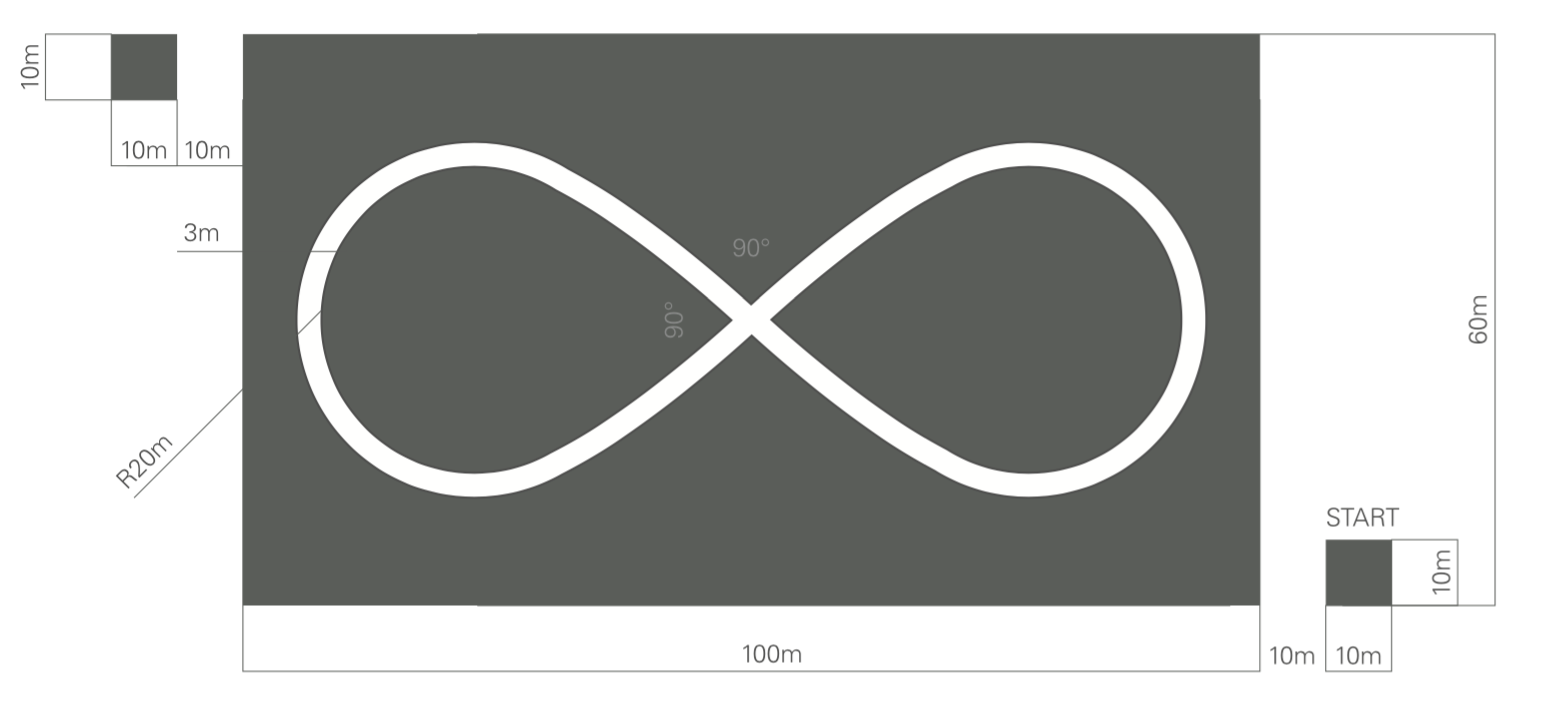
\includegraphics[width=1\textwidth]{img/arena.png}
    \caption{Arena of the challenge}
    \label{fig:arenachallenge}
\end{figure}

\subsection{Landing platform}
The landing platform is mounted on a ground vehicle of approximate dimensions $2.5m \times 1.5m \times 1.5m$ (length, width, height). The moving car starts at a constant speed of $15km/h$, it reduces the speed to $10km/h$ after 6 minutes and to $5 Km/h$ after 12 minutes.\\
The landing platform will be made of a ferrous surface to enable docking using magnetic or suction or other means.
It is a square of dimensions $1.5m \times 1.5m$, and approximately $1.5m$ above ground, positioned on the vehicle. 
The landing zone inside the landing area is a circle of diameter $1m$. The center of the circle is indicated by an X. The landing area, the landing zone and the marker X are shown in Figure \ref{fig:finalplatform}.
A landing is considered successful when a point of contact of the UAV is within the landing circle, with propulsion off and rotors not spinning.\\

\begin{figure}[!htbp]
    \centering
    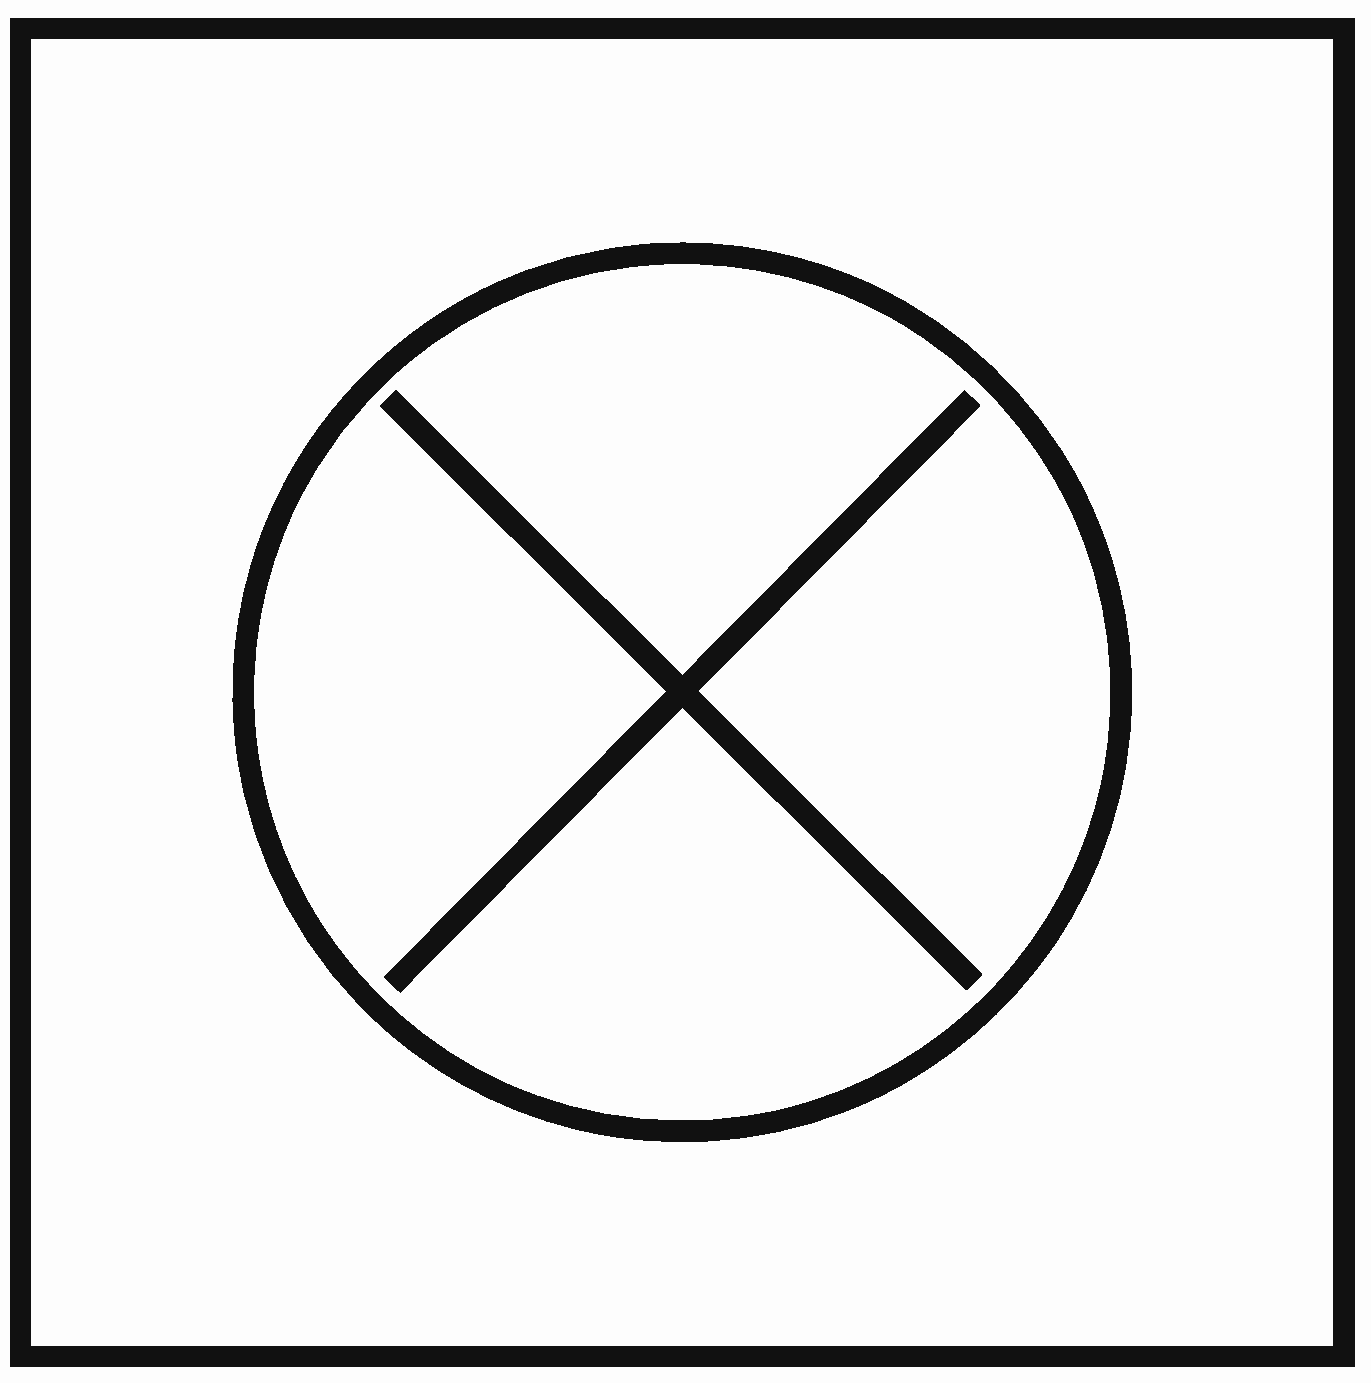
\includegraphics[width=0.3\textwidth]{img/base.pdf}
    \caption{Design of the platform in which the quadrotor must land on}
    \label{fig:finalplatform}
\end{figure}


